\documentclass[12pt,openright,twoside,french]{book}

\input philippe2013
\input philippe2013_activites

\pagestyle{empty}

\begin{document}

\TitreExo{\bsc{iv} - 1}{\'Equations du second degré \\ Application en économie}

L'entreprise Brillor fabrique et vend un détergent.\par
Le coût total journalier est donné par :
\[C(q) = 0,06q^2 + 0,1 q + 2,\] où la quantité $q$ est exprimée en tonne et varie de $1$ à $12$ tonnes.\par
La courbe représentative de $C$ est tracée ci-dessous.\par
On suppose que toute la fabrication est vendue.\medskip

\begin{enumerate}
    \item Aujourd'hui, l'entreprise a produit $9$ tonnes du produit. Quel en a été le coût ?
    \item Calculer $C(0)$. En donner une interprétation concrète.
    \item La recette journalière est donnée par $R(q) = 0,9q$.
        \begin{enumerate}
            \item Quelle est la recette obtenue pour $0$ tonnes vendues ?
            \item Quelle est la recette obtenue pour $9$ tonnes vendues ?
            \item Sur le repère ci-dessous, tracer la représentation graphique de la fonction $R$.
        \end{enumerate}
    \item Exprimer le bénéfice $B(q)$ pour $q \in \intervalleff{1}{12}$.
    \item Résoudre $B(q) = 0$. Arrondir à $10kg$ près par excès.\par Interpréter les résultats obtenus.
\end{enumerate}

\begin{center}
    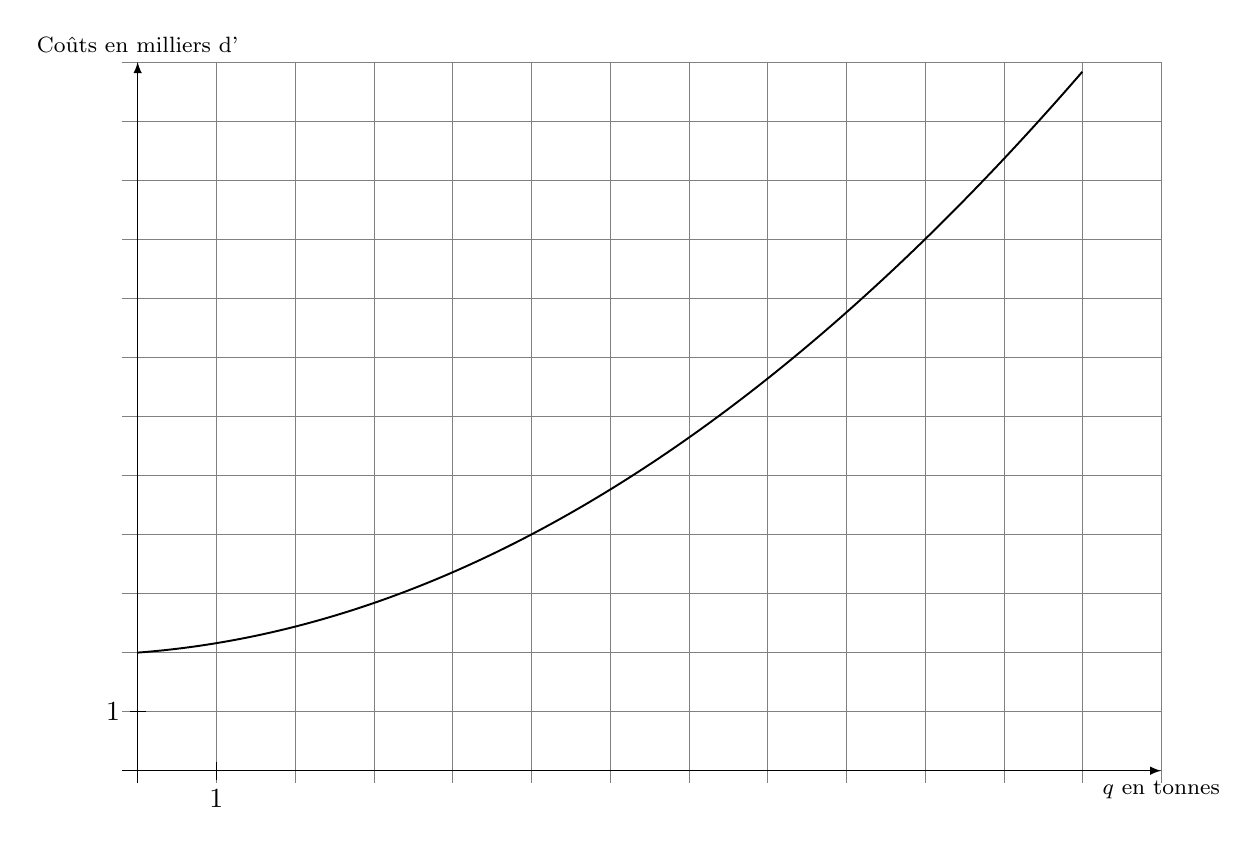
\begin{tikzpicture}[>=latex,yscale=0.75]
        \draw[help lines] (-0.2,-0.2) grid (13,12);
        \draw[->] (-0.2,0) -- (13,0) node[below] {\footnotesize $q$ en tonnes};
        \draw[->] (0,-0.2) -- (0,12) node[above] {\footnotesize Coûts en milliers d'\EUR{}};
        \draw[line width=0.7pt] plot[domain=0:12,samples=200] (\x,{0.06*(\x)^2 + 0.1*\x + 2});
        \draw (1,0.15)--(1,-0.15) node[below] {$1$};
        \draw (0.1,1)--(-0.1,1) node[left] {$1$};
    \end{tikzpicture}
\end{center}

\end{document} 